\begin{tikzpicture}[
    every node/.style={inner sep=0, outer sep=0},
]
    \node (img) at (0,0) {
        \includegraphics[width=\figurewidth]{figures/torque_tube_lines.png}
    };
    \begin{scope}[
        shift=(img.south west), % origin is lower left corner
        x={($(img.south east)-(img.south west)$)}, % x axis is lower side
        y={($(img.north west)-(img.south west)$)}] % y axis is left side
        % uncomment the following three lines to show a helper grid that helps
        % with finding coordinates
        % \draw[help lines, opacity=0.5, xstep=.01,ystep=.01] (0,0) grid (1,1);
        % \draw[thin, xstep=.1,ystep=.1] (0,0) grid (1,1);
        % \foreach \x in {0,...,9} { \node [anchor=north] at (\x/10,0) {0.\x}; }
        % \foreach \y in {0,...,9} { \node [anchor=east] at (0,\y/10) {0.\y}; }
        % draw stuff on image
        % (0, 0) is lower left corner, (1, 1) is upper right
        \node at (0.916,0.37) {
            \begin{tikzpicture}
                \draw[-latex, ultra thick, black, rotate=76] (0,0)
                arc[x radius = 2.6cm, y radius = 0.8cm, start angle= 60, end angle= -255];
            \end{tikzpicture}
        };

        \node at (0.123,0.705) {
            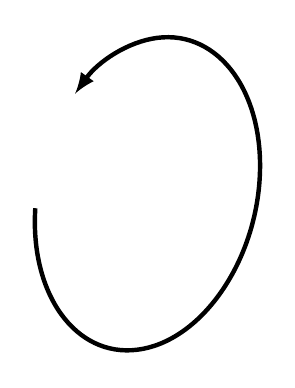
\begin{tikzpicture}
                \draw[-latex, ultra thick, black, rotate=76] (0,0)
                arc[x radius = 2.02cm, y radius = 1.385cm, start angle= -255, end angle= 60];
            \end{tikzpicture}
        };
    \end{scope}
\end{tikzpicture}